%
% 3dimagetemplate.tex
%
% (c) 2021 Prof Dr Andreas Müller, OST Ostschweizer Fachhochschule
%
\documentclass[tikz]{standalone}
\usepackage{times}
\usepackage{amsmath}
\usepackage{txfonts}
\usepackage[utf8]{inputenc}
\usepackage{graphics}
\usetikzlibrary{arrows,intersections,math,calc}
\usepackage{ifthen}
\begin{document}

\newboolean{showgrid}
\setboolean{showgrid}{false}
\def\breite{7}
\def\hoehe{4}

\def\achslabel{
	\node at (-1.75,-1.35) {$x$};
	\node at (1.8,-1.3) {$y$};
	\node at (0.7,1.1) {$z$};
}
\def\marke#1#2#3{
	\fill[color=white,opacity=0.7] ($#1+(-0.6,-0.2)$) rectangle +(1.2,0.4);
	\node[color=#3] at #1 {$#2\mathstrut$};
}
\definecolor{rot}{rgb}{0.8,0.4,0.6}
\definecolor{blau}{rgb}{0.4,0.6,0.8}
\begin{tikzpicture}[>=latex,thick]

% Povray Bild
\begin{scope}[xshift=-4.4cm]
\node at (0,0) {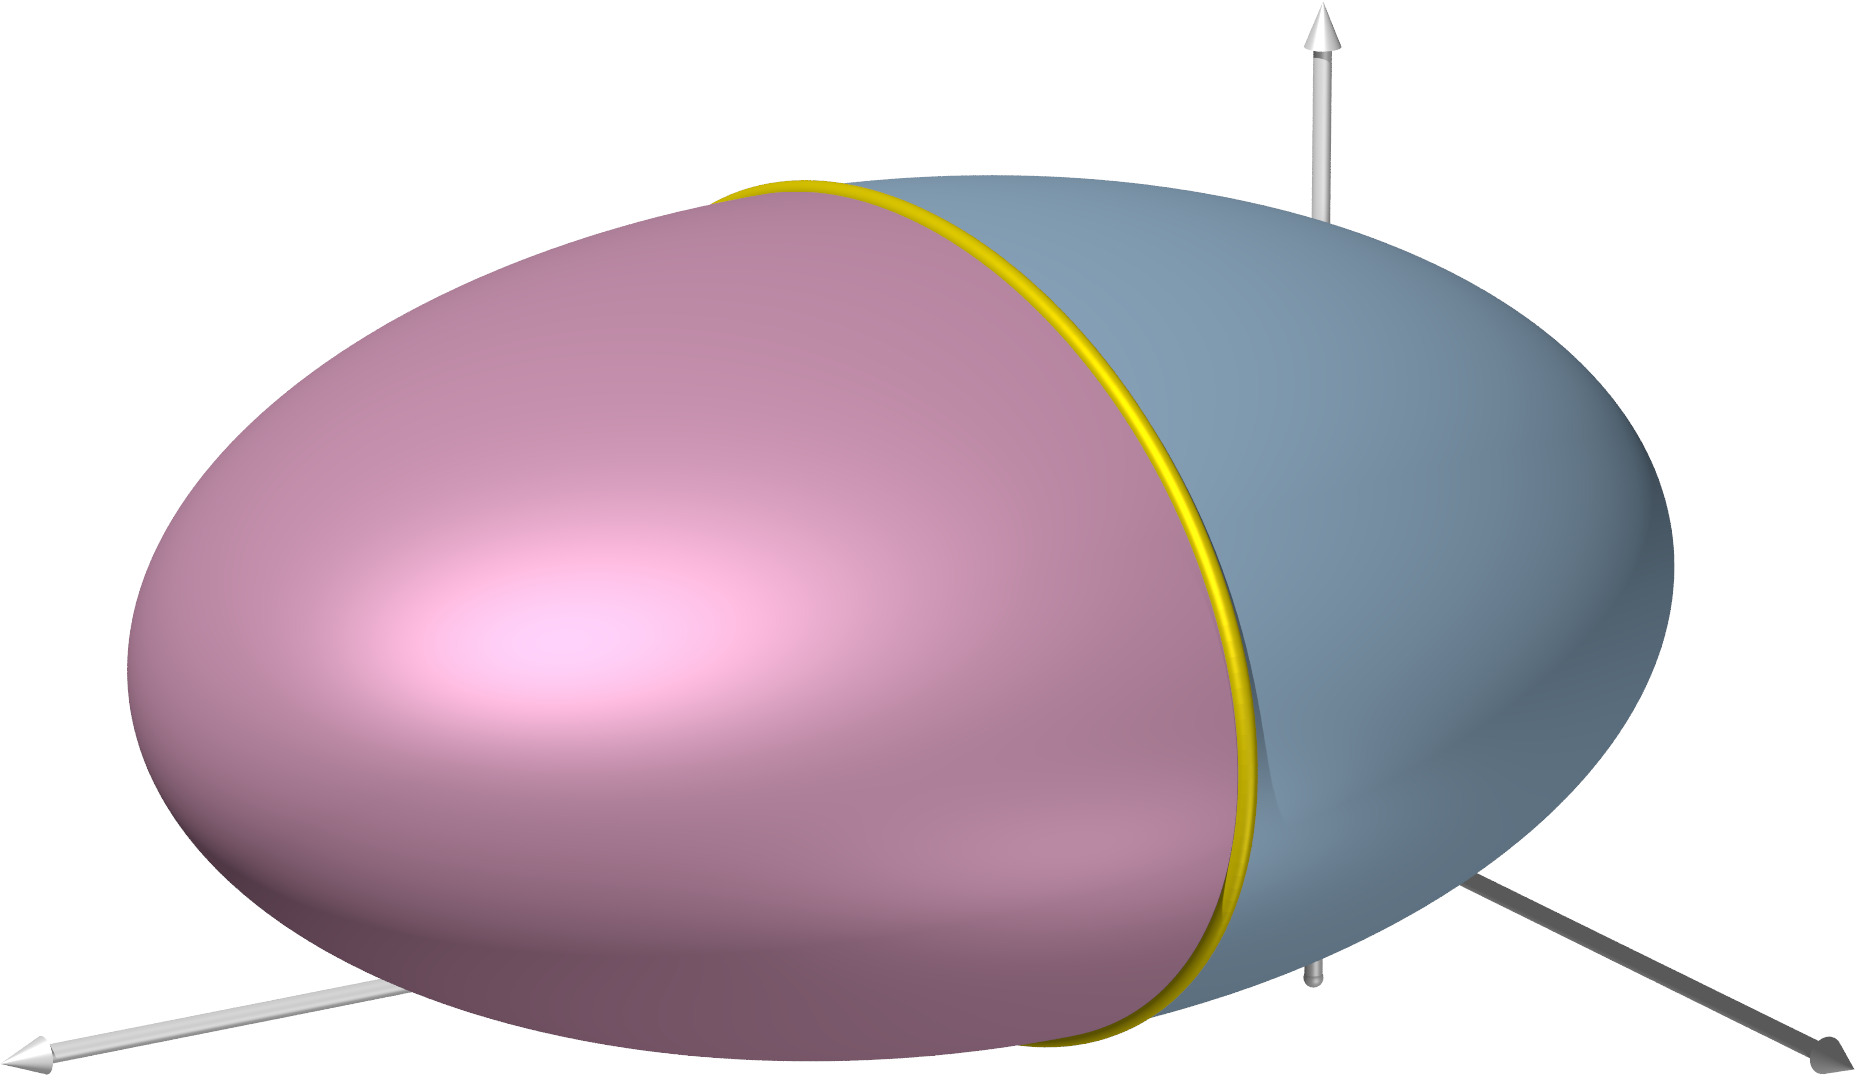
\includegraphics[width=4.2cm]{gaussx.jpg}};
\achslabel
\marke{(-0.7,-0.3)}{x_+(y,z)}{rot}
\marke{(1.4,0.1)}{x_-(y,z)}{blau}
\end{scope}

\begin{scope}
\node at (0,0) {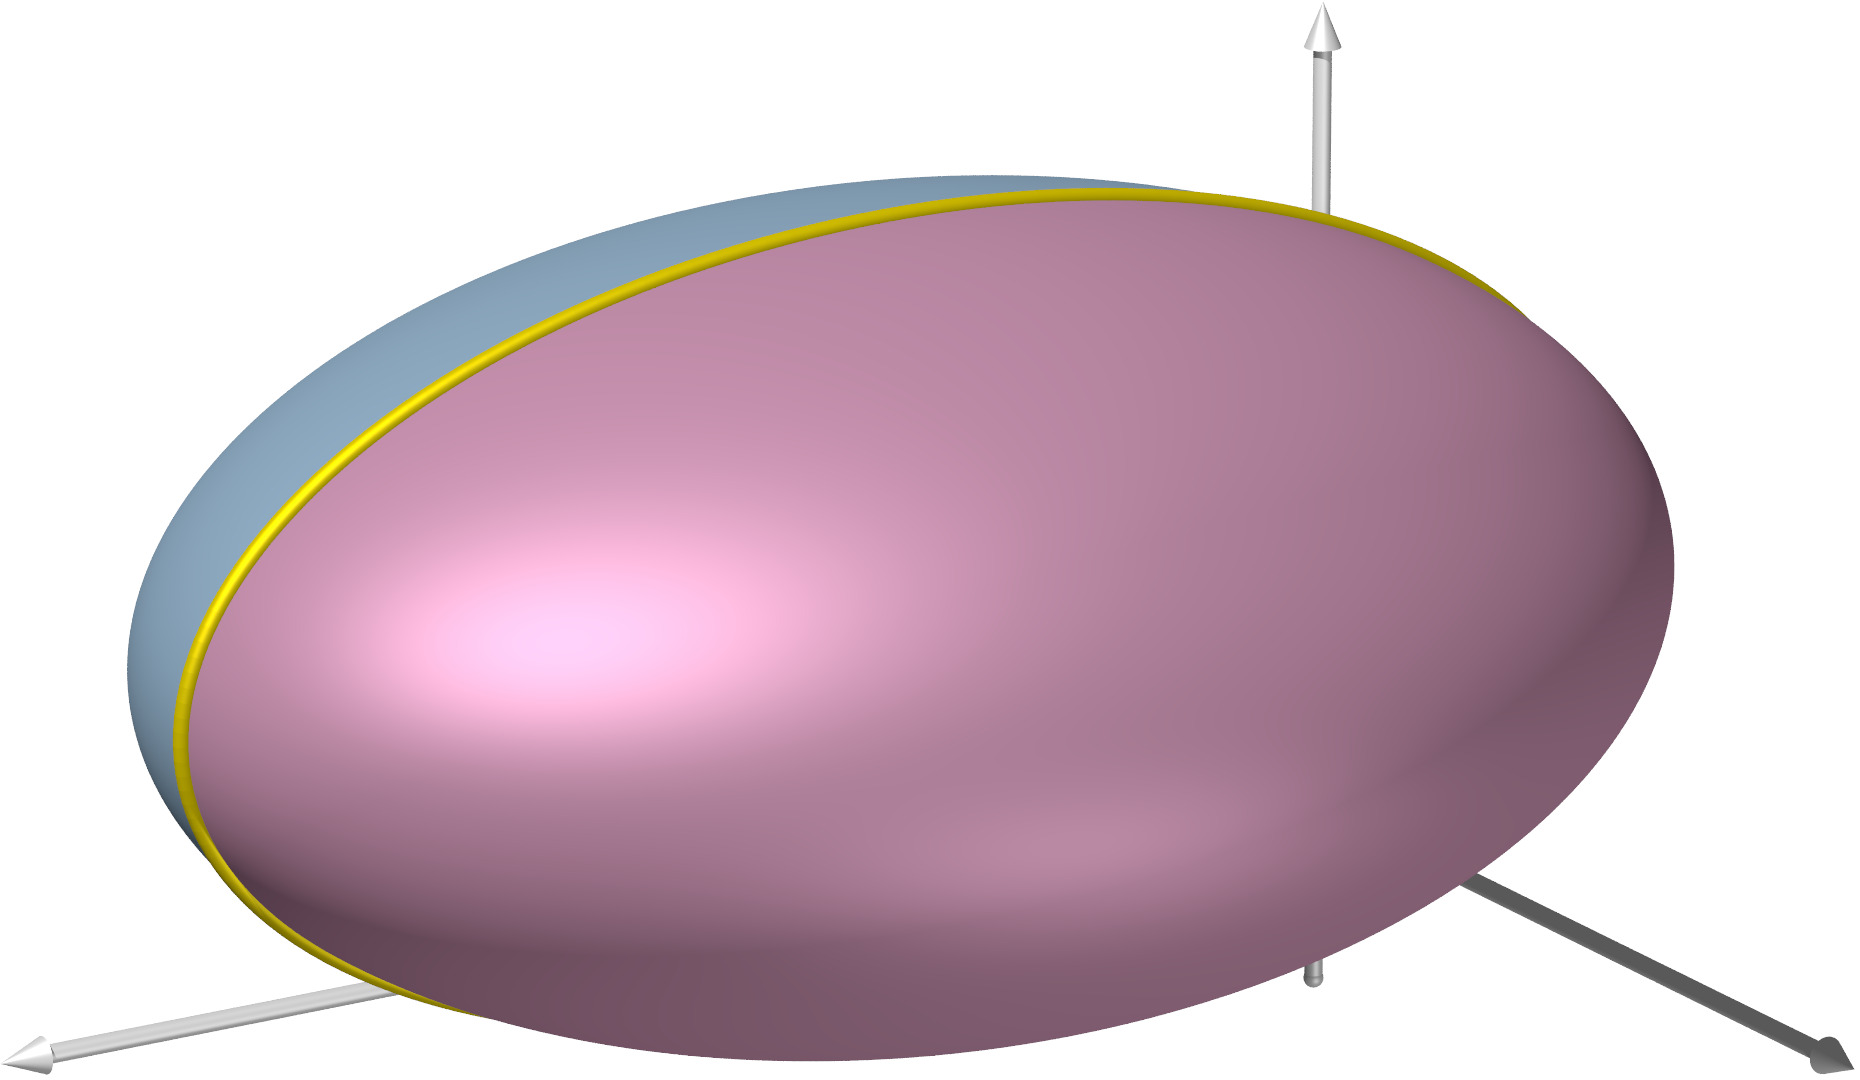
\includegraphics[width=4.2cm]{gaussy.jpg}};
\achslabel
\marke{(0.4,-0.3)}{y_+(x,z)}{rot}
\marke{(-1.4,0.7)}{y_-(x,z)}{blau}
\end{scope}

\begin{scope}[xshift=4.4cm]
\node at (0,0) {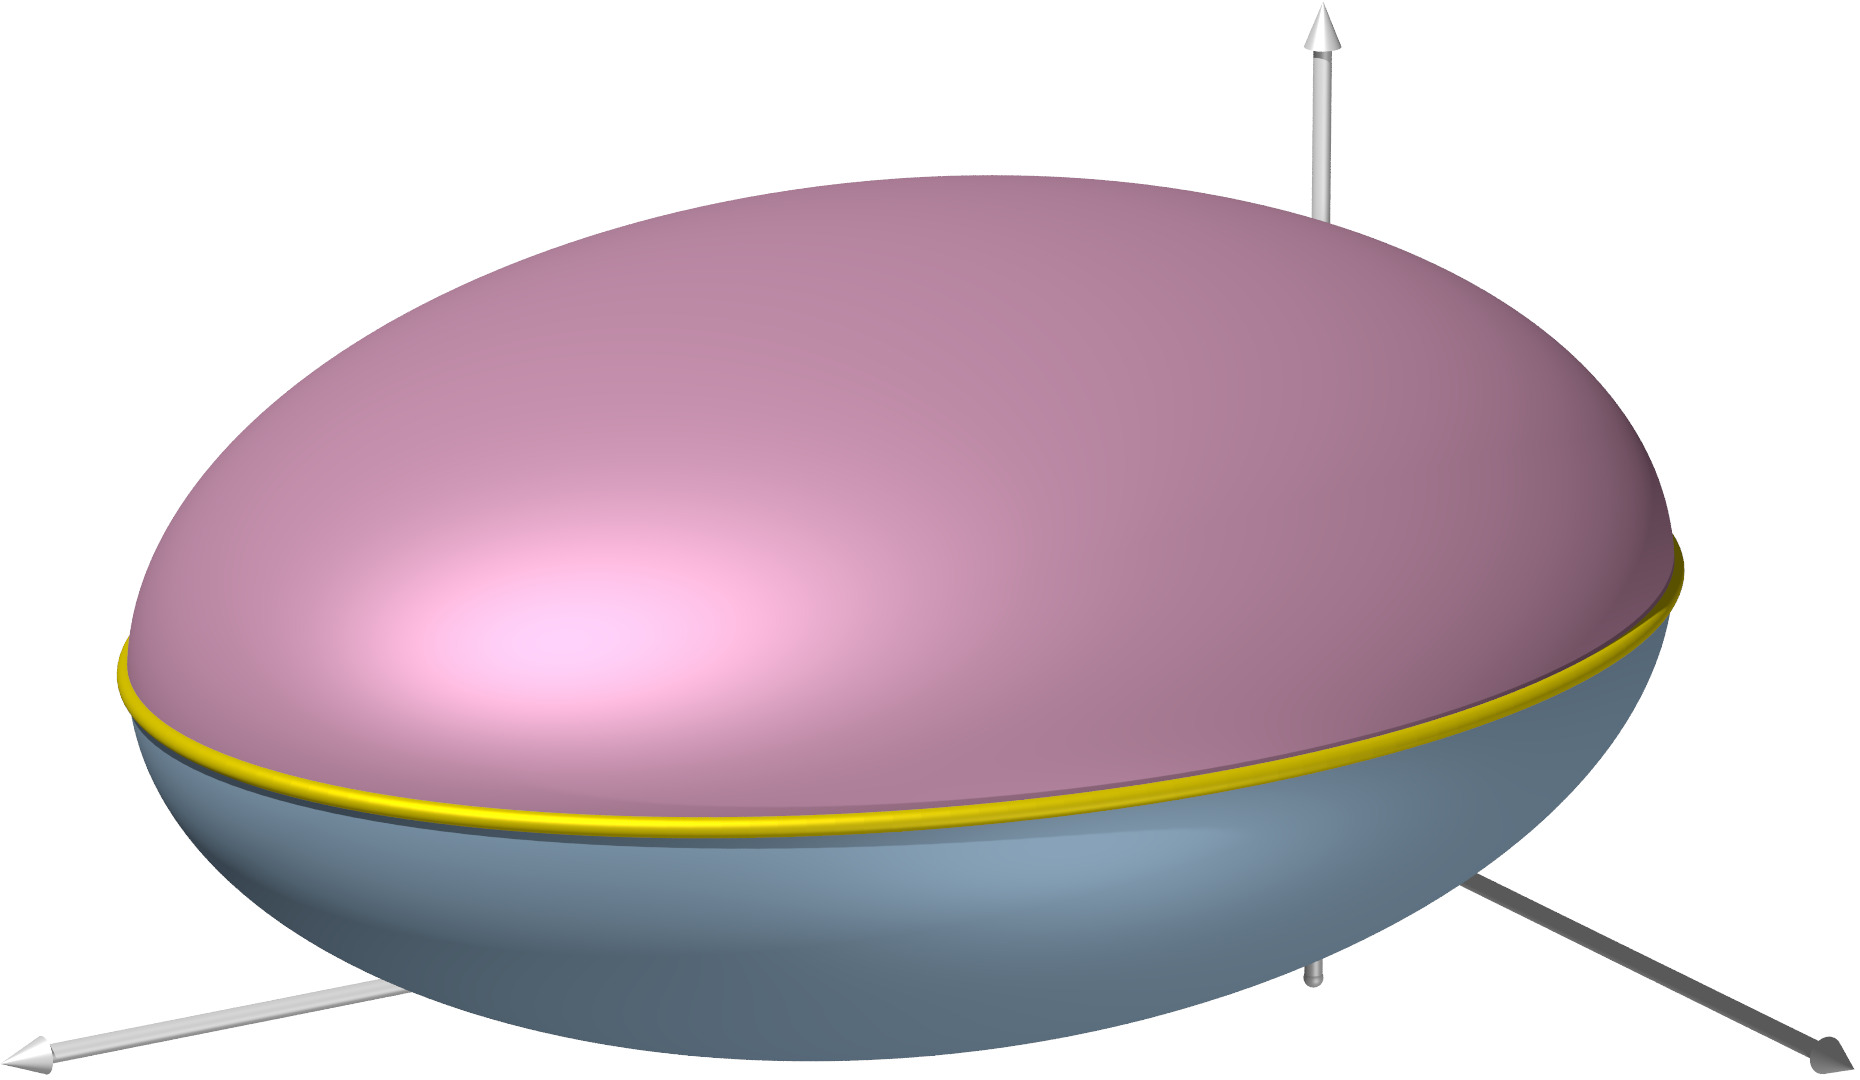
\includegraphics[width=4.2cm]{gaussz.jpg}};
\achslabel
\marke{(0.0,0.3)}{z_+(x,y)}{rot}
\marke{(-0.2,-0.95)}{z_-(x,y)}{blau}
\end{scope}

% Gitter
\ifthenelse{\boolean{showgrid}}{
\draw[step=0.1,line width=0.1pt] (-\breite,-\hoehe) grid (\breite, \hoehe);
\draw[step=0.5,line width=0.4pt] (-\breite,-\hoehe) grid (\breite, \hoehe);
\draw                            (-\breite,-\hoehe) grid (\breite, \hoehe);
\fill (0,0) circle[radius=0.05];
}{}

\end{tikzpicture}

\end{document}

